% Simplified planar reading for planning lecture P6 (TASKS.md D9), drafted
% from Bodily, Allen, and Killpack (ICRA 2017). Original wording and diagrams.
% Shared layout adapted from the instructor's ME 537 homework sources.
\documentclass[12pt,letterpaper]{article}
\usepackage{mathptmx}
\usepackage[T1]{fontenc}
\usepackage{xcolor,amsmath,amssymb,xurl,listings,enumitem,tikz}
\textwidth=6.5in
\textheight=9in
\oddsidemargin=0in
\evensidemargin=0in
\topmargin=0in
\headheight=0in
\headsep=0in
\parskip=0.08in
\parindent=0in
\setlist[enumerate]{itemsep=0.04in,topsep=0.04in}
\lstset{basicstyle=\ttfamily\footnotesize,breaklines=true,columns=fullflexible,
keepspaces=true,showstringspaces=false,aboveskip=0.04in,belowskip=0.04in}
\newcommand{\R}[2]{{}^{#1}\!R_{#2}}
\newcommand{\T}[2]{{}^{#1}\!T_{#2}}
\newcommand{\courseheader}[2]{%
\setlength{\fboxrule}{2pt}\setlength{\fboxsep}{2mm}%
\fcolorbox{black}{white}{\parbox{\dimexpr\linewidth-2\fboxsep-2\fboxrule\relax}{\centering\textbf{Introduction to Robotics Homework \##1 -- Draft}}}\par
\textbf{#2}\par}
\newcommand{\conventions}{Use right-handed rotations, column vectors, radians,
and meters. $\R{A}{B}$ maps coordinates from frame $B$ into frame $A$;
$\T{A}{B}$ also includes the origin of $B$ expressed in $A$.}
\newcommand{\submission}{\textbf{Submit:} labeled hand derivations and sketches,
your changed Python source files, the requested numerical/visual evidence,
and an AI-use statement (including ``none'' if applicable). Show your reasoning
before using code to check hand calculations. Public checks are intentionally
limited. The instructor supplies the deadline and submission destination.}

\newcommand{\readingheader}[1]{%
\setlength{\fboxrule}{2pt}\setlength{\fboxsep}{2mm}%
\fcolorbox{black}{white}{\parbox{\dimexpr\linewidth-2\fboxsep-2\fboxrule\relax}{\centering\textbf{Introduction to Robotics Reading -- Draft}}}\par
\textbf{#1}\par}
\usepackage{needspace}
% Compact section headings that never sit alone at the bottom of a page.
\newcommand{\heading}[1]{\par\needspace{5\baselineskip}\smallskip{\large\textbf{#1}}\par}
\begin{document}
\readingheader{Following a tool path with a redundant arm: inverse kinematics branching}

\textbf{Source.} This reading is a simplified, planar version of
D.~M.~Bodily, T.~F.~Allen, and M.~D.~Killpack, ``Motion Planning for Mobile
Robots Using Inverse Kinematics Branching,'' \emph{IEEE International
Conference on Robotics and Automation (ICRA)}, 2017, pp.~5043--5050. We keep
the central idea and drop the parts that need tools beyond this course
(Section~6 lists them). The example code is
\path{examples/position_only_branching.py}.

\heading{1. The task}
Painting, sanding, or wiping a wall asks the tool to pass through a sequence
of positions $p_1,\dots,p_k$ along a path. Often only the tool's
\emph{position} matters, not its orientation. A planar arm with $n>2$
revolute joints is then redundant: every reachable point can be reached by
infinitely many configurations $q\in\mathbb{R}^n$. We want a sequence
$q_1,\dots,q_k$ in which
\begin{itemize}\setlength{\itemsep}{0pt}
\item configuration $q_i$ puts the tool at $p_i$;
\item neighboring configurations are close, so the motion is smooth;
\item every joint stays inside its limits, preferably away from them; and
\item no link touches an obstacle.
\end{itemize}

\heading{2. Why stepping along the path with IK can fail}
The direct approach solves IK for $p_1$, then uses that answer as the starting
guess for $p_2$, and so on. Each solve uses the damped pseudo-inverse step
from lecture,
\begin{equation}
\Delta q = J^T\left(JJ^T+\lambda^2 I\right)^{-1} e,\qquad e = p - p_{\text{tool}}(q),
\end{equation}
where $J$ is the first two rows of \texttt{jacob\_planar(q)}. Each solve only
looks at its own target. The first answer commits the arm to a family of
shapes, for example elbow down, and later targets are reached by continuing
that family, even if it runs through an obstacle or into a joint stop.
Nothing earlier in the sequence knew what was coming.

\begin{center}
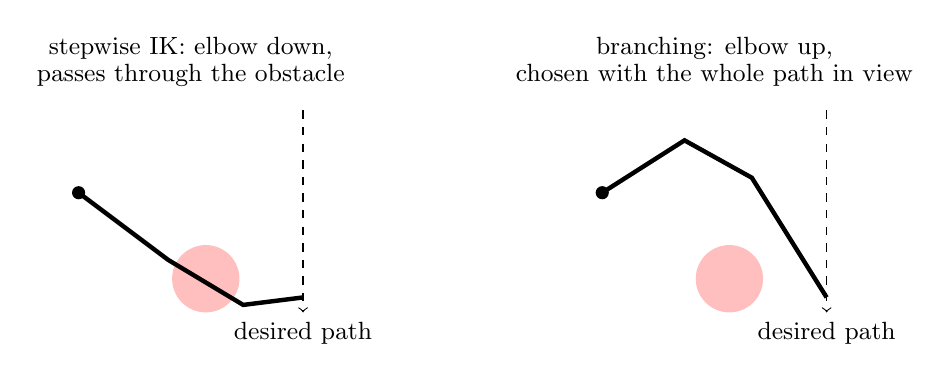
\begin{tikzpicture}[scale=0.95]
\begin{scope}
\draw[dashed,->] (3,1.1)--(3,-1.6) node[below]{\small desired path};
\fill[red!25] (1.7,-1.15) circle (0.45);
\draw[line width=1.6pt] (0,0)--(1.2,-0.9)--(2.2,-1.5)--(3,-1.4);
\fill (0,0) circle (2.5pt);
\node[align=center] at (1.5,1.75) {\small stepwise IK: elbow down,\\[-2pt]\small passes through the obstacle};
\end{scope}
\begin{scope}[xshift=7cm]
\draw[dashed,->] (3,1.1)--(3,-1.6) node[below]{\small desired path};
\fill[red!25] (1.7,-1.15) circle (0.45);
\draw[line width=1.6pt] (0,0)--(1.1,0.7)--(2.0,0.2)--(3,-1.4);
\fill (0,0) circle (2.5pt);
\node[align=center] at (1.5,1.75) {\small branching: elbow up,\\[-2pt]\small chosen with the whole path in view};
\end{scope}
\end{tikzpicture}
\end{center}

\heading{3. Branching: solve for every configuration at once}
Make $k$ \emph{virtual} copies of the arm, all sharing one fixed base, and
assign copy $i$ the target $p_i$. The unknown is now one long vector holding
a small change for every copy,
$\Delta = [\Delta q_1;\ \Delta q_2;\ \dots;\ \Delta q_k]$ with $kn$ entries.
Each iteration chooses $\Delta$ to make a sum of squared terms small. Each
term is linear in $\Delta$ (we linearize the tool position with $J_i$, the
first two rows of \texttt{jacob\_planar}$(q_i)$):
\begin{align}
&\text{reach the targets:} && \textstyle\sum_{i=1}^{k} \|J_i\Delta q_i - e_i\|^2, \quad e_i = p_i - p_{\text{tool}}(q_i)\\
&\text{smooth motion:} && \textstyle\kappa\sum_{i=1}^{k-1}\|(q_i+\Delta q_i)-(q_{i+1}+\Delta q_{i+1})\|^2\\
&\text{stay near joint centers:} && \textstyle\beta\sum_{i=1}^{k}\|q_i+\Delta q_i-q_c\|^2\\
&\text{stay off obstacles:} && \textstyle c\sum_{\text{near links}}\Big(\tfrac{\epsilon-d}{\epsilon}\Big)^2\big(n^T J_{\text{link}}\Delta q_i-(\epsilon-d)\big)^2
\end{align}
In term~(5), $d$ is the distance from a link to the obstacle's edge, the term
is used only when $d<\epsilon$, $n$ is the unit direction away from the
obstacle, and $J_{\text{link}}$ is the Jacobian of the link's closest point
(columns for joints beyond that link are zero). It asks that point to move
outward by $\epsilon-d$, more strongly the closer it is.

Adding damping $\lambda^2\|\Delta\|^2$, the whole cost is one least-squares
problem,
\begin{equation}
\min_{\Delta}\ \|A\Delta-b\|^2 ,
\end{equation}
where each term contributes rows to $A$ and $b$ (multiply a term's rows by
the square root of its weight). For $k=3$ the reach and smoothness rows look
like
\[
A=\begin{bmatrix}
J_1&0&0\\0&J_2&0\\0&0&J_3\\
\sqrt{\kappa}I&-\sqrt{\kappa}I&0\\
0&\sqrt{\kappa}I&-\sqrt{\kappa}I\\
\multicolumn{3}{c}{\vdots}
\end{bmatrix},\qquad
b=\begin{bmatrix}e_1\\e_2\\e_3\\-\sqrt{\kappa}(q_1-q_2)\\-\sqrt{\kappa}(q_2-q_3)\\\vdots\end{bmatrix}.
\]
The block-diagonal part is $k$ separate IK problems. The smoothness rows
couple neighbors, and that coupling is what gives each copy ``global
context'': a copy near the obstacle pulls its neighbors toward a shape that
works for it, and the whole family moves together. With one copy and only
terms (2) and the damping, the solution is exactly the damped pseudo-inverse
step (1) (question 1).

After solving, the example limits each joint's step, tries step lengths
$\alpha\in\{1,\ 0.5,\ 0.25\}$ and keeps the one that lands closest to the
targets (a simple line search), and clamps every joint to its limits.

\heading{4. Turning down the secondary weights}
Large $\kappa$ and $\beta$ early on make the copies spread out smoothly and
stay in comfortable shapes, but they also hold the tools back from their
targets. The paper therefore decays these weights: whenever the total
position error stops improving, multiply $\kappa$ and $\beta$ by a factor
$\rho<1$ (the example halves them). By the end the problem is almost pure
IK, but started from a well-organized, collision-free set of shapes. The
obstacle weight $c$ stays constant so the copies keep their distance.

\heading{5. Running the example}
\begin{lstlisting}
python -m examples.position_only_branching --show
python -m examples.position_only_branching --kappa 0 --show
python -m examples.position_only_branching --no-obstacle --show
\end{lstlisting}
The arm has four 0.2~m links and $k=10$ targets on a vertical line at
$x=0.55$~m, with a circular obstacle below the path. The top row of the
figure shows the copies branching out over the iterations. The bottom row
compares the stepwise IK baseline with the final branching result and plots
each joint angle against the copy index. In the default run the branching
copies reach their targets within about $10^{-4}$~m after roughly 100
iterations and clear the obstacle by about 6~cm, while the stepwise baseline
passes 9~cm into it.

\heading{6. What the full paper adds}
\begin{itemize}\setlength{\itemsep}{0pt}
\item \textbf{Full poses in 3D.} Targets are positions and orientations; the
error is a twist from the matrix logarithm, with weights choosing how much
orientation matters. Our version sets the orientation weight to zero.
\item \textbf{A quadratic program.} Joint stops and step limits are exact
inequality constraints ($A\Delta\le b$) solved with a QP solver, rather than
the clamping used here.
\item \textbf{The base is optimized too.} All copies share a base whose pose
is an extra unknown, so the planner also chooses where to park a mobile base
or lift platform.
\item \textbf{Manipulability.} A term rewards motion that increases
$\sqrt{\det(JJ^T)}$, keeping the arm away from singular shapes.
\item \textbf{Refinement.} After solving with a moderate $k$, the planner
solves again between neighboring copies to produce a finely spaced path.
\item \textbf{Real robots.} It planned painting and sanding motions for an
8-joint, pneumatically actuated soft arm built by Pneubotics, and motions
for an arm on a planetary rover model, in a few seconds.
\end{itemize}
It is still a \emph{local} method: a maze-like scene can trap it. The authors
suggest seeding it with a sampling-based planner such as RRT-Connect and then
using branching to shorten and smooth the result.

\heading{Questions}
\begin{enumerate}
\item With $k=1$ and only term (2) plus damping $\lambda^2\|\Delta q\|^2$,
set the gradient to zero and show the minimizer is
$\Delta q=(J^TJ+\lambda^2I)^{-1}J^Te$. Then show this equals step (1).
\item For $k=10$ and $n=4$, how many unknowns does $\Delta$ have, and how
many rows do terms (2)--(4) and the damping add to $A$? Why is $A$ mostly
zeros, and why does that matter for larger problems?
\item Run the example with \texttt{-{}-kappa 0}. Find the pair of neighboring
copies whose joint angles jump, and explain what the robot would have to do
between those two configurations.
\item Run it with \texttt{-{}-no-obstacle}. Which family of shapes does
branching choose now, and why does the default run choose differently?
\end{enumerate}
\end{document}
